%%%%%%%%%%%%%%%%%%%%%%%%%%%%%%%%%%%%%%%%%%%%%%%%%%%%%%%%%%%%%%%%%%%%%%%%%%%%%%%%
% Soutenance de projet - Fichier modèle pour présentations Beamer
%%%%%%%%%%%%%%%%%%%%%%%%%%%%%%%%%%%%%%%%%%%%%%%%%%%%%%%%%%%%%%%%%%%%%%%%%%%%%%%%
\documentclass{beamer}
\usepackage[utf8]{inputenc}
\usepackage[francais]{babel}
\usepackage[T1]{fontenc}
\usepackage{textcomp}
\usepackage{relsize}
\usepackage{amssymb}
\usepackage{framed}


%%% THÈME TORINO AVEC MINIFRAMES MODIFIÉES - NÉCESSITE FICHIERS SPÉCIAUX
\usetheme[pageofpages=sur,% String used between the current page and the
                         % total page count.
          alternativetitlepage=true,% Use the fancy title page.
          titlepagelogo=logo,% Logo for the first page.
          titleline=true,
          watermark=watermark,% Watermark used in every page.
          watermarkheight=100px,% Height of the watermark.
          watermarkheightmult=4,% The watermark image is 4 times bigger
                                % than watermarkheight.
          ]{Torino}
\useoutertheme[subsection=true]{miniframes2}
\usecolortheme{freewilly}
%%% FIN DU SECOND THÈME

% nouvelle commande pour un joli nom
\newcommand{\nom}[1]{\textsc{#1}}

% commande pour une zolie ligne
\newcommand{\ligne}[1][1pt]{
  \par\noindent
  \rule[.5ex]{\linewidth}{#1}\par}

% \0
\newcommand{\slz}{$\backslash0$}

% commande pour un message réseau
\newcommand{\netmessage}[5]{\small \begin{framed}
\texttt{Message} \emph{#1} \texttt{- #2 - #3 $\rightarrow$ #4}\\\noindent
\rule{\linewidth}{0.4pt}

\footnotesize\noindent\texttt{#5}

\end{framed}}

%%% TITRE DE PAGE
\title{Contextd Capture}
\subtitle{Capture d'activité système pour PIGA-SYSTRANS}
\author{Dimitri~Gressin \and Timothée~Ravier}
\institute{ENSI de Bourges}
\date{20 janvier 2011}

%%% POUR AVOIR UN PLAN QUI S'AFFICHE QUAND ON CHANGE DE SOUS-SECTION
\AtBeginSection[ ]
{
 \begin{frame}<beamer>
   \frametitle{Plan}
   \tableofcontents[currentsection]
  \end{frame}
}
\NoAutoSpaceBeforeFDP

\begin{document}

%%% LA PAGE DE TITRE, ON PEUT Y APPLIQUER DES OPTIONS COMME INSTITUTE CI-DESSOUS
{
	\framenumberoff
	\watermarkoff
	\institute{École Nationale Supérieure d'Ingénieurs de Bourges} % Vire le champ institut sur cette page
	\begin{frame}
	\titlepage
	\end{frame}
}

\section{Introduction}
\begin{frame}
\frametitle{Context\{e|d\}}
\begin{itemize}
	\item Commande différents systèmes de sécurité pour autoriser une application à effectuer certaines actions
	\item Pour fonctionner, il doit avoir connaissance :
		\begin{itemize}
			\item des accès aux fichiers
			\item des noms de domaine des sites visités
		\end{itemize}
\end{itemize}
\end{frame}

\begin{frame}
\frametitle{Présentation du sujet}
\begin{itemize}
	\item Intercepter les appels système
	\item Récupérer des informations telles que PID, fichiers ouverts, socket créée, etc.
	\item Envoyer ces informations dans l'espace utilisateur au démon contextd
	\item Retourner la réponse de contextd au noyau pour débloquer l'appel système
\end{itemize}
\end{frame}

\section{Systemtap}
\begin{frame}
\frametitle{Systemtap}
\begin{center}
	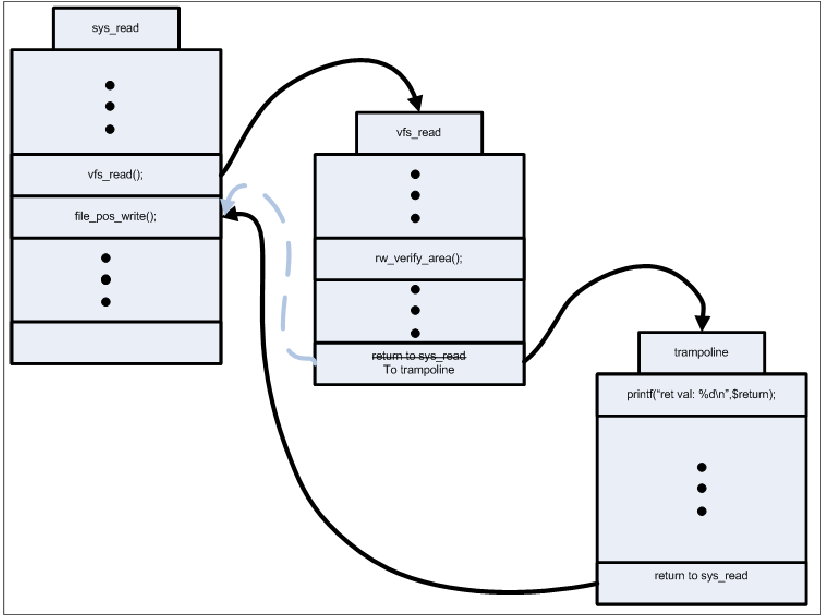
\includegraphics[scale=0.25]{kretprob.png}
\end{center}
\end{frame}

\begin{frame}
\frametitle{Systemtap}
\begin{itemize}
	\item Les scripts sont exécutés après les appels système
	\item Impossibilité de suspendre un appel système
	\item Les données accessibles sont inexploitables
\end{itemize}
~\\
\textbf{Systemtap ne répondait absolument pas à nos besoins}

\end{frame}

\section{Linux Security Modules}
\begin{frame}
\frametitle{}
	\begin{itemize}
		\item Ce sont des modules noyau
		\item Ils permettent de "hooker" les appels système
		\item Ils permettent d'interdire dynamiquement des appels système
	\end{itemize}
~\\	
\textbf{Les modules LSM répondent tout à fait à notre problématique}
\end{frame}

\begin{frame}
\frametitle{Schéma}
\begin{center}
	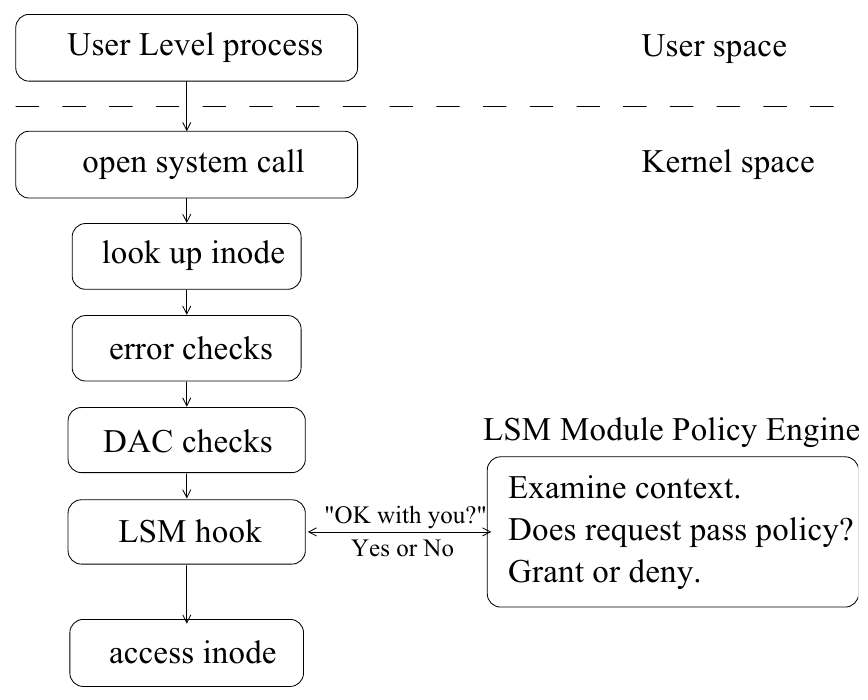
\includegraphics[scale=0.30]{lsm1.png}
\end{center}
\end{frame}

\begin{frame}
\frametitle{Notre travail}
\begin{itemize}
	\item Création du module LSM\\
	\item Ajout dans le mode de configuration standard du noyau\\
	\item Manipulation de deux "hooks"\\
	\begin{itemize}
		\item file permission : appelé à chaque fois qu'un fichier est ouvert
		\item socket bind : appelé à chaque création de socket (à venir)
	\end{itemize}
\end{itemize}
\textbf{Hooks principaux en ce qui concerne contextd}\\
% \textbf{Évite de passer par ULOG pour la partie "réseau"}\\
\end{frame}

\section{Objectifs suivants}
\begin{frame}
\frametitle{Prochaines étapes}
\begin{enumerate}
	\item Communication entre les espaces noyau et utilisateur :
	\begin{itemize}
		\item[-] Via des sockets unix ?
		\item[-] Via un proc filesystem ?
		\item[-] Via un chardev ?
		\item[-] Via des appels système !
	\end{itemize}
	\item Démon qui fera le lien entre l'espace noyau et contextd
	\item Eventuellement remplacé à terme par un plugin contextd
\end{enumerate}
\end{frame}

\begin{frame}
\frametitle{Appels système}
\begin{center}
	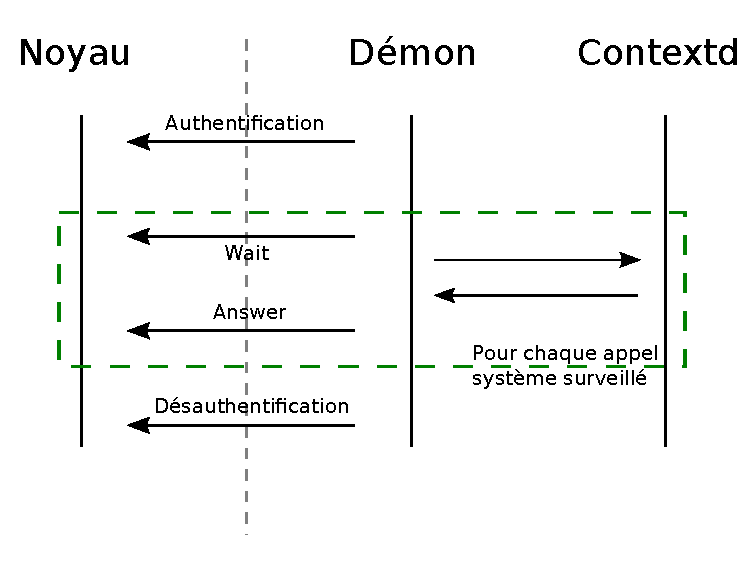
\includegraphics[scale=0.75]{global.pdf}
\end{center}
\end{frame}

\section{Conclusion}
\begin{frame}
\frametitle{Conclusion}
\begin{itemize}
	\item Certains objectifs sont atteints
	\item Seule une petite partie du projet est visible pour l'instant
\end{itemize}
\end{frame}

\end{document}
